\documentclass[12pt, twoside]{article}
\usepackage[francais]{babel}
\usepackage[T1]{fontenc}
\usepackage[latin1]{inputenc}
\usepackage[left=7mm, right=7mm, top=7mm, bottom=7mm]{geometry}
\usepackage{float}
\usepackage{graphicx}
\usepackage{array}
\usepackage{multirow}
\usepackage{amsmath,amssymb,mathrsfs}
\usepackage{soul}
\usepackage{textcomp}
\usepackage{eurosym}
 \usepackage{variations}
\usepackage{tabvar}

\pagestyle{empty}

\begin{document}

\begin{flushleft}
NOM PRENOM: \ldots \ldots \ldots \ldots \ldots \ldots \ldots \ldots \ldots
 
\bigskip

\end{flushleft}

\begin{center}
{\fbox{$5^{e}1$ \qquad \qquad \textbf{\Large{Contr�le de cours 3 (sujet 1)}}
\qquad \qquad 14/12/2009}}
\end{center}



\bigskip

\textit{Remarque: Tout le contr�le est � faire sur cette feuille. Laisser vos
traits de constructions (pour le rep�re).}


\enskip


\ul{Exercice 1}: Comparer les nombres suivants:

\begin{center}
-2 \ldots \ldots -4

\enskip

+7 \ldots \ldots 7,03

\enskip

-5,6 \ldots \ldots -5,7

\enskip

-1,3 \ldots \ldots +1,3
\end{center}


\bigskip


\ul{Exercice 2}: 

\begin{center}
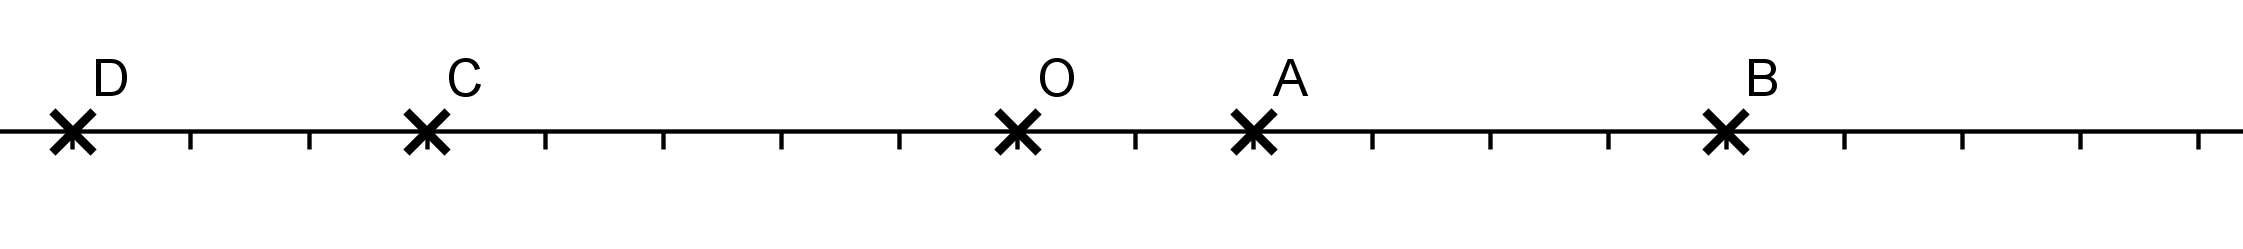
\includegraphics[width=14cm]{images/droite1.png}
\end{center}


\begin{enumerate}
  \item Quelle est l'abscisse du point B?  \qquad \quad \ldots \ldots \ldots
  \ldots \ldots
  
  
  \item Quelle est l'abscisse du point C?    \qquad \quad \ldots \ldots \ldots
  \ldots \ldots
  
  \item Quelle est l'abscisse du point D?    \qquad \quad \ldots \ldots \ldots
  \ldots \ldots
  
  \item Placer sur cette droite les points E(+3) et F(-1).
\end{enumerate}


\bigskip


\ul{Exercice 3}: 



\begin{center}
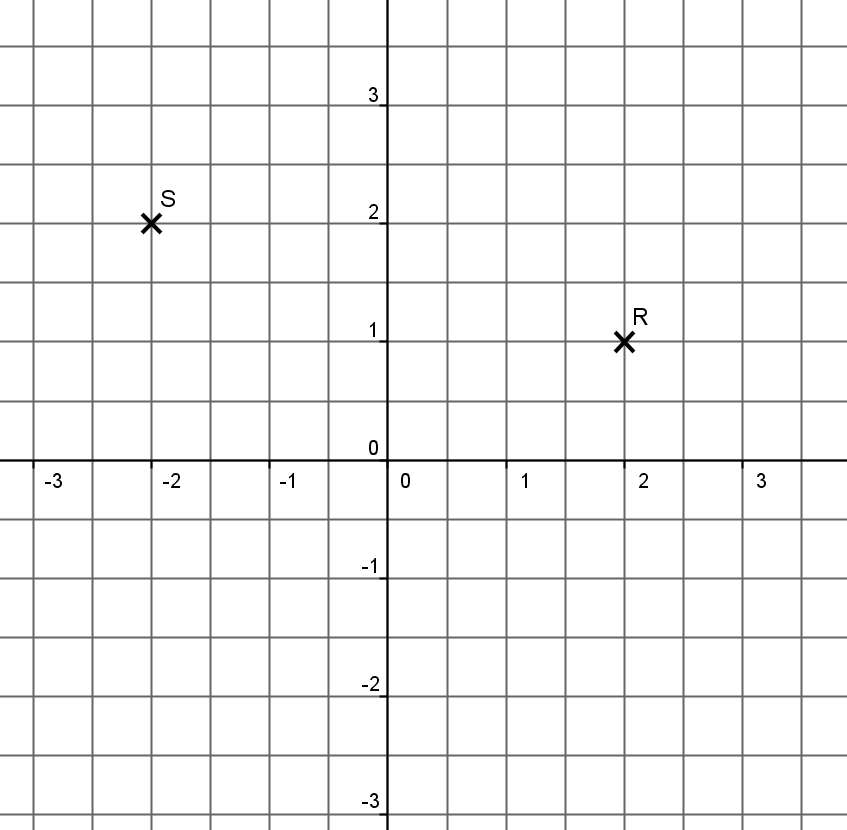
\includegraphics[width=10cm]{images/repere1.png}
\end{center}


\begin{enumerate}
  \item Donner les coordonn�es du point R. \qquad \quad \ldots \ldots \ldots
  \ldots \ldots 
  
  \item Donner les coordonn�es du point S.  \qquad \quad \ldots \ldots \ldots
  \ldots \ldots  
  
  \item Placer le point U(-3;-2).
  
  \item Placer le point T(+1,5;-2,5).
\end{enumerate}



\pagebreak



\begin{center}
{\fbox{$5^{e}1$ \qquad \qquad \textbf{\Large{Contr�le de cours 3 (sujet 2)}}
\qquad \qquad 14/12/2009}}
\end{center}



\bigskip

\textit{Remarque: Tout le contr�le est � faire sur cette feuille. Laisser vos
traits de constructions (pour le rep�re).}


\enskip


\ul{Exercice 1}: Comparer les nombres suivants:

\begin{center}
+12 \ldots \ldots 12,07

\enskip

-6 \ldots \ldots -3

\enskip

+1,2 \ldots \ldots -1,2

\enskip

-2,3 \ldots \ldots -2,4
\end{center}


\bigskip


\ul{Exercice 2}: 

\begin{center}
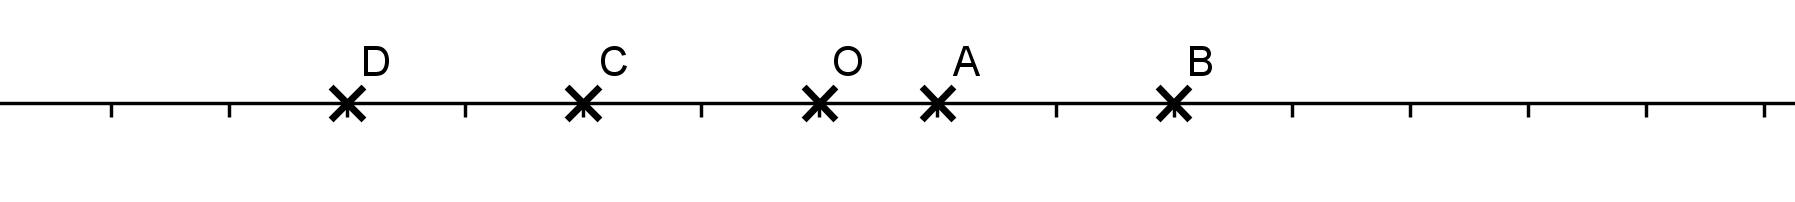
\includegraphics[width=14cm]{images/droite2.png}
\end{center}


\begin{enumerate}
  \item Quelle est l'abscisse du point B?  \qquad \quad \ldots \ldots \ldots
  \ldots \ldots
  
  
  \item Quelle est l'abscisse du point C?    \qquad \quad \ldots \ldots \ldots
  \ldots \ldots
  
  \item Quelle est l'abscisse du point D?    \qquad \quad \ldots \ldots \ldots
  \ldots \ldots
  
  \item Placer sur cette droite les points E(+2) et F(-1,5).
\end{enumerate}


\bigskip


\ul{Exercice 3}: 



\begin{center}
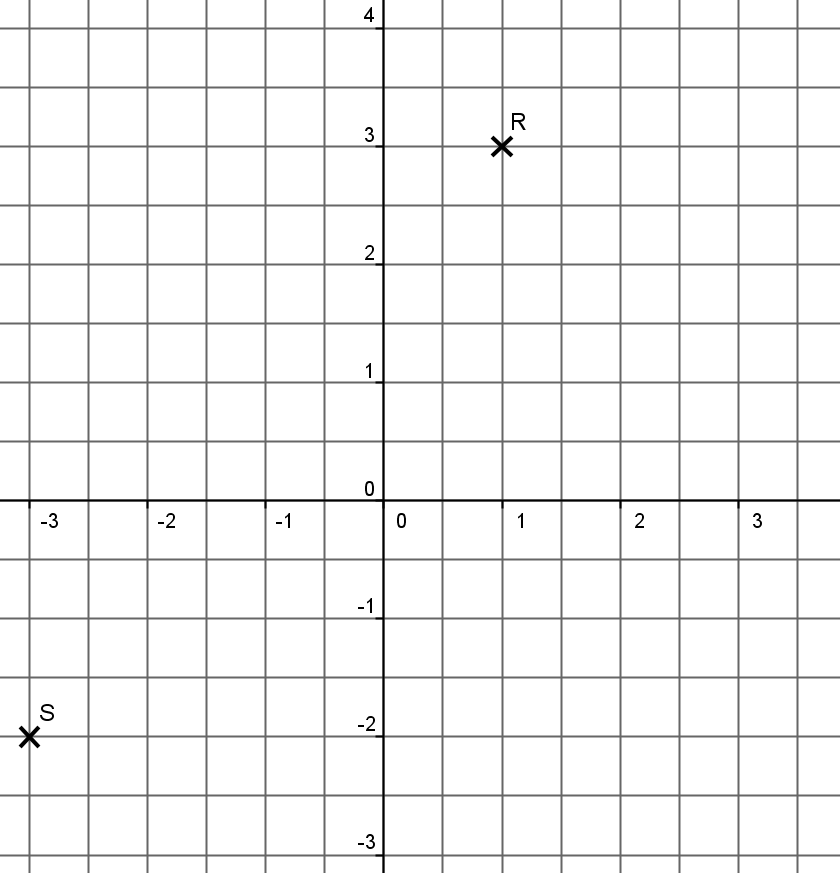
\includegraphics[width=10cm]{images/repere2.png}
\end{center}


\begin{enumerate}
  \item Donner les coordonn�es du point R. \qquad \quad \ldots \ldots \ldots
  \ldots \ldots 
  
  \item Donner les coordonn�es du point S.  \qquad \quad \ldots \ldots \ldots
  \ldots \ldots  
  
  \item Placer le point U(+2;-1).
  
  \item Placer le point T(-1,5; +3,5).
\end{enumerate}


\pagebreak


\begin{flushleft}
NOM PRENOM: \ldots \ldots \ldots \ldots \ldots \ldots \ldots \ldots \ldots
 
\bigskip

\end{flushleft}

\begin{center}
{\fbox{$5^{e}2$ \qquad \qquad \textbf{\Large{Contr�le de cours 3 (sujet 1)}}
\qquad \qquad 14/12/2009}}
\end{center}



\bigskip

\textit{Remarque: Tout le contr�le est � faire sur cette feuille. Laisser vos
traits de constructions (pour le rep�re).}


\enskip


\ul{Exercice 1}: Comparer les nombres suivants:

\begin{center}
-2 \ldots \ldots -4

\enskip

+7 \ldots \ldots 7,03

\enskip

-5,6 \ldots \ldots -5,7

\enskip

-1,3 \ldots \ldots +1,3
\end{center}


\bigskip


\ul{Exercice 2}: 

\begin{center}
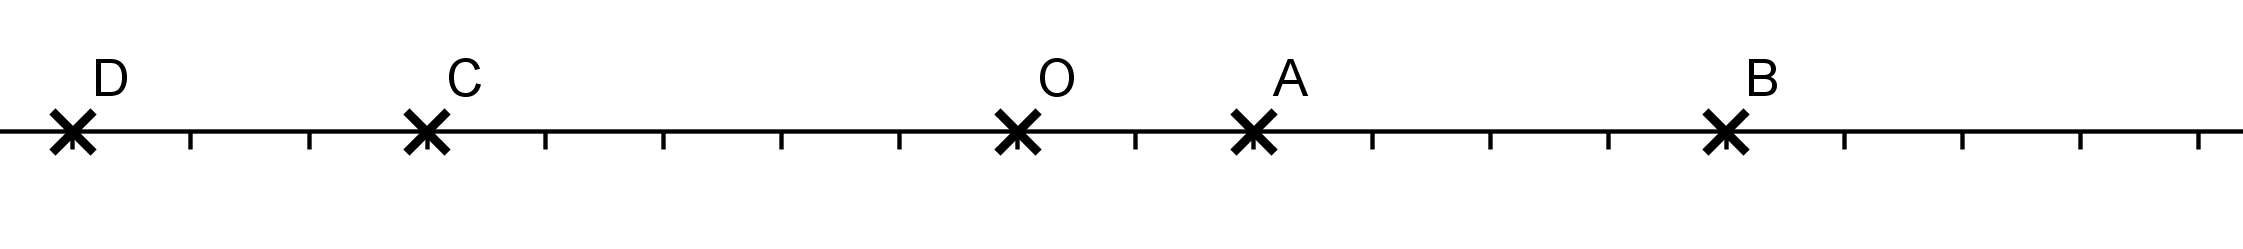
\includegraphics[width=14cm]{images/droite1.png}
\end{center}


\begin{enumerate}
  \item Quelle est l'abscisse du point B?  \qquad \quad \ldots \ldots \ldots
  \ldots \ldots
  
  
  \item Quelle est l'abscisse du point C?    \qquad \quad \ldots \ldots \ldots
  \ldots \ldots
  
  \item Quelle est l'abscisse du point D?    \qquad \quad \ldots \ldots \ldots
  \ldots \ldots
  
  \item Placer sur cette droite les points E(+3) et F(-1).
\end{enumerate}


\bigskip


\ul{Exercice 3}: 



\begin{center}
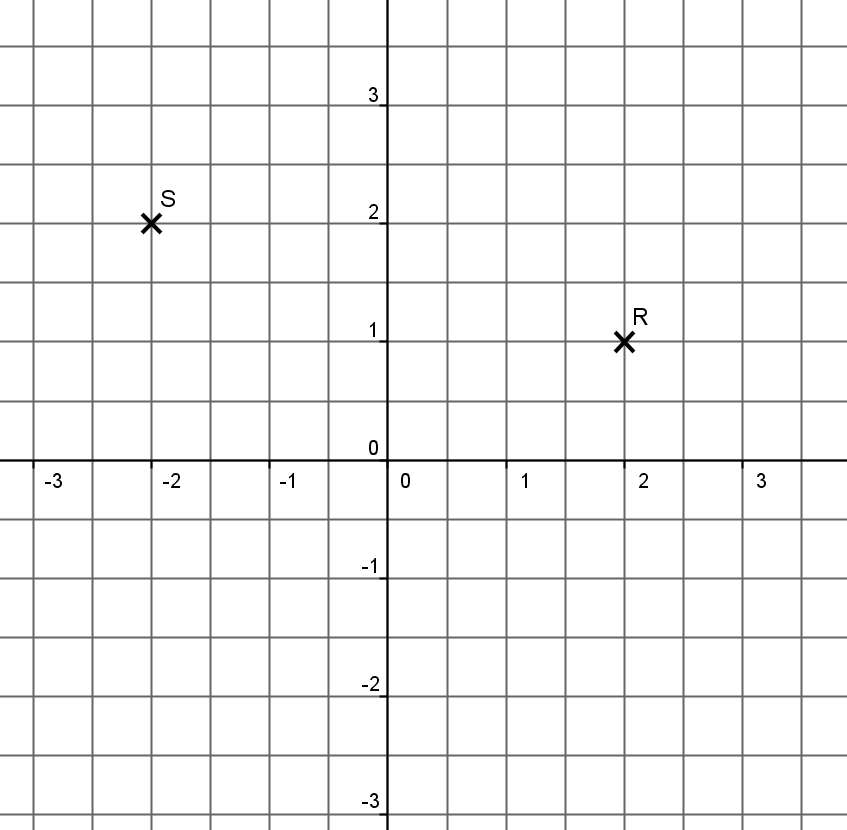
\includegraphics[width=10cm]{images/repere1.png}
\end{center}


\begin{enumerate}
  \item Donner les coordonn�es du point R. \qquad \quad \ldots \ldots \ldots
  \ldots \ldots 
  
  \item Donner les coordonn�es du point S.  \qquad \quad \ldots \ldots \ldots
  \ldots \ldots  
  
  \item Placer le point U(-3;-2).
  
  \item Placer le point T(+1,5;-2,5).
\end{enumerate}



\pagebreak



\begin{center}
{\fbox{$5^{e}2$ \qquad \qquad \textbf{\Large{Contr�le de cours 3 (sujet 2)}}
\qquad \qquad 14/12/2009}}
\end{center}



\bigskip

\textit{Remarque: Tout le contr�le est � faire sur cette feuille. Laisser vos
traits de constructions (pour le rep�re).}


\enskip


\ul{Exercice 1}: Comparer les nombres suivants:

\begin{center}
+12 \ldots \ldots 12,07

\enskip

-6 \ldots \ldots -3

\enskip

+1,2 \ldots \ldots -1,2

\enskip

-2,3 \ldots \ldots -2,4
\end{center}


\bigskip


\ul{Exercice 2}: 

\begin{center}
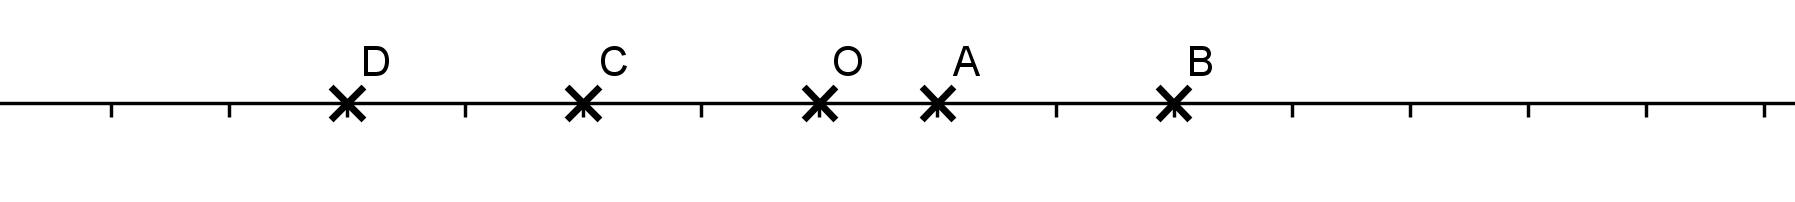
\includegraphics[width=14cm]{images/droite2.png}
\end{center}


\begin{enumerate}
  \item Quelle est l'abscisse du point B?  \qquad \quad \ldots \ldots \ldots
  \ldots \ldots
  
  
  \item Quelle est l'abscisse du point C?    \qquad \quad \ldots \ldots \ldots
  \ldots \ldots
  
  \item Quelle est l'abscisse du point D?    \qquad \quad \ldots \ldots \ldots
  \ldots \ldots
  
  \item Placer sur cette droite les points E(+2) et F(-1,5).
\end{enumerate}


\bigskip


\ul{Exercice 3}: 



\begin{center}
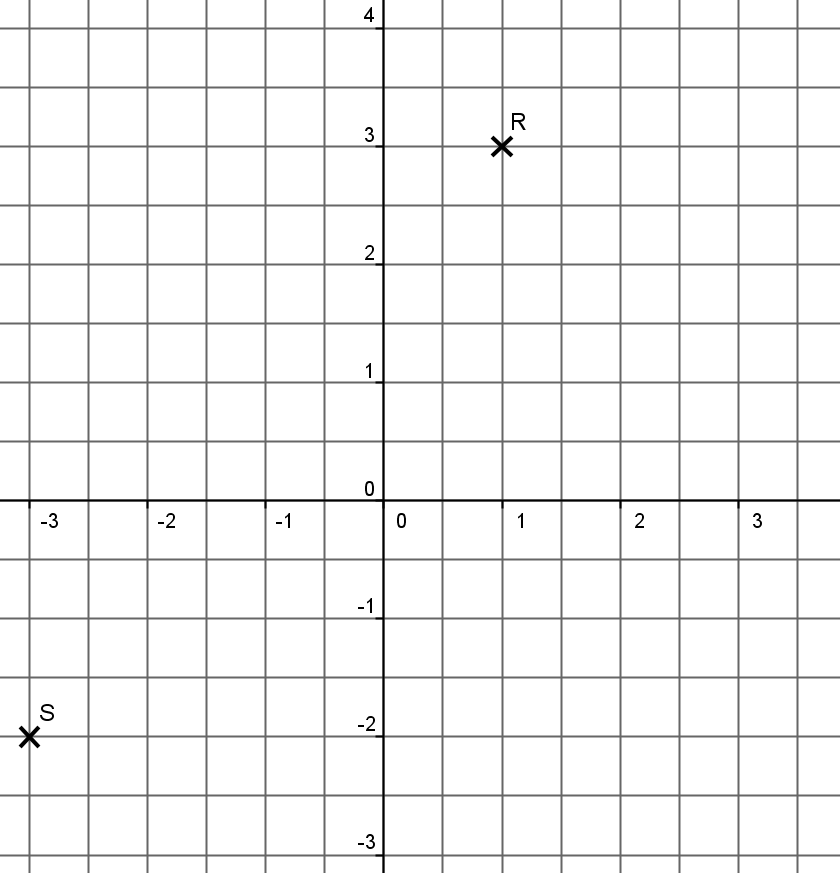
\includegraphics[width=10cm]{images/repere2.png}
\end{center}


\begin{enumerate}
  \item Donner les coordonn�es du point R. \qquad \quad \ldots \ldots \ldots
  \ldots \ldots 
  
  \item Donner les coordonn�es du point S.  \qquad \quad \ldots \ldots \ldots
  \ldots \ldots  
  
  \item Placer le point U(+2;-1).
  
  \item Placer le point T(-1,5; +3,5).
\end{enumerate}
\end{document}
